% Document class `report-template` accepts either project-plan or final-report option in
% []. This will change the title page as necessary.
% \documentclass[project-plan]{report-template}
\documentclass[final-report]{report-template}

% Packages I use in my report.
\usepackage{graphicx}
\usepackage{amsmath}
\usepackage{blindtext}
\usepackage{array}  
\usepackage{caption}
\usepackage{float}
\usepackage{rotating}

% Directory where I saved my figures.
\graphicspath{{./figures/}}

% Metadata used for the title page - please modify.
\university{Imperial College London}
\department{Department of Earth Science and Engineering}
\course{MSc in Applied Computational Science and Engineering}
\title{OpenWeather ChatAgent: Design and Implementation of an AI Weather Assistant System}
\author{Fangze Liu}
\email{fangze.liu24@imperial.ac.uk}
\githubusername{esemsc-fl724}
\supervisors{Prof. Christopher Pain\\
             Dr. Olga Buskin}
\repository{https://github.com/ese-ada-lovelace-2024/irp-fl724}

\begin{document}

\maketitlepage  % generate title page

\section*{AI Acknowledgement Statement}
I used OpenAI’s ChatGPT‑4o (https://chat.openai.com/) to support my learning and understanding of large language models (LLMS), as well as to debug and test the code of my projects. This generative AI tool supported my learning process, but the submitted work is my own and it reflects my own understanding and effort as I declared by signing the Academic Integrity Declaration.

% Abstract
\section*{Abstract}


% Introduction section
\section{Introduction}
\subsection{Background and Problem Description}
Weather, as the most critical environmental information after time and place, has a direct and far-reaching impact on people's daily lives. It is crucial to obtain timely and accurate weather information. However, traditional weather query systems mostly use template-based responses or keyword matching, which are unable to understand the diversified expressions of user's natural language, and are difficult to adapt to the increasingly complex query needs of users. As a result, building an AI Weather Assistant System powered by Large Language Models (LLMs) can significantly improve the user experiences.

In recent years, with the rapid development of LLMs in natural language processing, more and more users have started to use conversational LLMs like ChatGPT (OpenAI, 2023)~\cite{OpenAI2023} for various queries. However, many user questions require knowledge beyond what a pre-trained LLM can store internally.~\cite{Zhang2023} For example, a user might ask, "What’s the weather like in London right now?" Clearly, such tasks require accessing real-time data through external APIs.~\cite{Chadha2024} The ability to interact with tools is a key step in the evolution of LLMs from passive text generators to action-capable AI agents.

Nevertheless, applying LLMs to real-world weather queries presents several challenges, such as: how to understand the user's intention, how to call the APIs in a structured way to obtain the external data; and how to semantically process the returned data. Additional concerns such as error handling, multi-model compatibility, and asynchronous task execution further increase system complexity.


\subsection{Significance}
but also serve as a practical paradigm for engineering applications of LLMs that can be extended to other domains.

Weather services are fundamental for human safety, productivity, and planning, especially in urban and climate-sensitive areas. However, existing weather systems struggle to meet the rising expectations for personalized, real-time, and context-aware weather information. Traditional APIs or mobile apps often lack natural conversation capabilities and adaptability to user-specific needs.

This project demonstrates a practical engineering application of LLMs — not as passive question-answering bots, but as intelligent, action-capable agents capable of real-time data retrieval, semantic reasoning, and adaptive response generation. By integrating the OpenWeather API with LLM-powered tools and coordinating them via the Model Context Protocol (MCP), the project delivers a flexible, modular, and intelligent solution for real-world weather interactions.

More importantly, this system showcases how state-of-the-art AI technologies — including Function Calling, ReAct-style tool orchestration, user memory, multilingual output, and vector-based retrieval (RAG) — can be combined in a production-grade weather assistant. These design patterns can be extended to many other agent-based use cases such as finance, health, and education, thus presenting broader implications beyond weather applications.

\subsection{Review of Existing Work}


\subsection{Objectives and Expected Deliverables}
Therefore, this project aims to build an LLM-based AI weather agent system that can understand natural language queries, retrieve real-time weather data via the OpenWeather API~\cite{OpenWeatherAPI}, and generate informative and coherent replies to provide users with real and accurate weather data and related information.



% Another section
\section{Methodology}
\subsection{OpenWeather API}

This project uses the OpenWeather One Call API to obtain current weather conditions, hourly/daily forecasts, historical data, and weather alerts. By calling the endpoint at \url{https://api.openweathermap.org/data/3.0/onecall}~\cite{OpenWeatherAPI} and providing the geographic coordinates of a city, the system retrieves structured meteorological data to supply the agent with real-time external information support.


\subsection{Function Calling and Tool Invocation}
Due to inherent technical limitations, large language models (LLMs) cannot directly communicate with external tools. To solve this problem, OpenAI introduced Function Calling in March 2023. This technique enables LLMs to call external tools by creating an intermediary function that bridges the model’s request and the external API, so that the model has the ability to call external tools. Function Calling~\cite{Liu2024}~\cite{Gim2024} is an important foundation to promote the evolution of the LLMs from a dialogue tool to an AI Agent,  which are capable of autonomously perceiving the environment, making decisions, and taking actions.

In this project, Function Calling enables the model to automatically generate structured parameters and call the OpenWeather API based on user requests, so that the system not only understands and generates natural language, but also calls specific APIs or tools to complete more complex tasks based on user needs. (Figure 1)

Function Calling not only improves the accuracy and personalization of the model's response, but also supports a “perception–action–feedback” loop, which enables dynamic execution of complex tasks. To simplify this process, we plan to explore coordination libraries (e.g., LangChain~\cite{LangChainIntro}), which provides modular support for tool-based LLM agents.~\cite{Anthonio2024}


% Figure
\begin{figure}[H]
    \begin{center}
        
\includegraphics[width=0.6\textwidth]{latex/figures/function calling.png}
    \end{center}
    \caption{\label{fig:function calling} Flowchart of Function Calling Execution}
\end{figure}

\subsection{MCP Protocol Integration}
Although traditional Function Calling enables large language models (LLMs) to invoke external tools, the lack of standardized specifications across different vendors often leads to high costs in function definition, API adaptation, and long-term maintenance, making the development process complex.

To address this challenge, Anthropic released the Model Context Protocol (MCP) in November 2024~\cite{Anthropic2024MCP}, introducing a standardized and distributed architecture consisting of a Client and a Server (Figure 2). With a unified specification, the development efficiency can be greatly improved.~\cite{Hou2025}~\cite{Luo2025}

Overall, MCP offers standardized interfaces, supports distributed and asynchronous execution, and provides a robust developer ecosystem, which fits the real-world business needs. In this project, we plan to explore the MCP protocol to improve interface compatibility and response performance, and lay the foundation for multi-model collaboration and complex task scheduling.

% Figure
\begin{figure}[H]
  \centering
  \fcolorbox{white}{white}{
    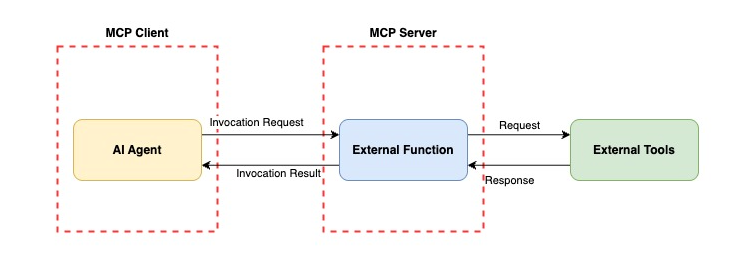
\includegraphics[width=0.9\textwidth]{figures/MCP.png}
  }
  \caption{Structure of the MCP Protocol}
  \label{fig:mcp}
\end{figure}

\subsection{Considerations and Limitations}
Although extensive literature and project reviews have been conducted, the methodology section currently only outlines a preliminary system architecture, as many practical challenges may arise during development. For example, although Function Calling has the disadvantage of inconsistent format and long code, it integrates well with AI agents and can simplify system testing. The MCP protocol seems to have all the advantages, but in fact it sends a large amount of context to the LLM, and if the performance of the LLM is not good enough, there may be side effects. Additional features such as context retrieval or user profiling may also need the introduction of Retrieval-Augmented Generation (RAG)~\cite{GaoYunfan2023}. Therefore, some methods have been marked as 'exploratory' to indicate that they are options that can be investigated further.

\newpage
\section{Deliverable}
Expected deliverables of this project:
	
\begin{enumerate}
  \item \textbf{System Prototype}
  \begin{itemize}
    \item Build an AI Weather Agent system based on OpenAI model and OpenWeather API~\cite{Cao2024}, which supports users to query real-time weather and weather report in natural language.

  \end{itemize}

  \item \textbf{Baseline Module Based on Function Calling}
  \begin{itemize}
    \item Use OpenAI’s Function Calling mechanism to construct tool functions, achieving structured integration between the LLM and the OpenWeather API.

  \end{itemize}

  \item \textbf{MCP protocol (Exploratory)}
  \begin{itemize}
    \item Implement a basic MCP client–server architecture to decouple the LLM from tool modules, supporting asynchronous task execution.

  \end{itemize}


  \item \textbf{Functional prototype}
  \begin{itemize}
    \item Develop a user-friendly frontend interface that supports natural language weather queries.
  \end{itemize}

  \item \textbf{Documentation \& Deployment Package}
  \begin{itemize}
    \item Provide comprehensive documentation, including system architecture diagrams, module specifications, a deployment guide, and API integration instructions.
  \end{itemize}

  \item \textbf{Optional Extensions (Exploratory)}
  \begin{itemize}
    \item Investigate integration with other LLMs (e.g., Gemini, DeepSeek) to evaluate multi-model compatibility.
    \item Explore context memory modules for maintaining user preferences and chat history.~\cite{LDAgent}
    \item Optionally extend support to historical weather data queries or knowledge-augmented generation (e.g., RAG)~\cite{GaoYunfan2023}~\cite{Jeong2024}. Further literature review is required to assess feasibility.
  \end{itemize}
\end{enumerate}




% References
\newpage
\bibliographystyle{plain}
\bibliography{references}  % BibTeX references are saved in references.bib

\end{document}          

